% !TEX root = ~/OpenFOAM/antoniopucciarelli-9/run/LABS/thermochemical_CFD/main.tex

\section{Final assignment -- $\mathtt{LabAssignment}$}
    
    \renewcommand{\thepage}{\arabic{page}}
    \setcounter{page}{\thelastPage}
    
    This last case treats the analysis of the 3D combustor. 

    The main difference among this case and the 2D cases is the computational cost related to the additional coordinate of study. Convergence parameters are set up in order to reduce the computational time and ensuring good results. 

    \subsection{Problem setup}
    \subsubsection{Boundary conditions}
    The main difference between the 2D case is the fact that there is no more the \verb|frontAndBack| patch. The \verb|frontAndBack| patch is changed with \verb|outerWalls| patch. 
    Because it is no more a 2D problem, the \verb|outerWalls| does not use the \verb|empty| type for the boundary conditions on every variables' dictionary. 

    \cprotect\subsubsection{\verb|fvModels|}
    This dictionary activates \textit{only} the lagrangian spray modeling. The liquid film modeling is not activated due to the computational resources available.
    \begin{lstlisting}[caption = $\mathtt{combustorReaction/constant/fvModels}$ activates only lagrangian spray model and the bouyancy forces., label = list:fvModels]
            buoyancyForce
            {
                type    buoyancyForce;
            }

            clouds
            {
                type    clouds;
                libs    ("liblagrangianParcel.so");
            }

            //surfaceFilm
            //{
            //    type    surfaceFilm;
            //    libs    ("libsurfaceFilmModels.so");
            //}
    \end{lstlisting}
    
    \cprotect\subsubsection{\verb|chemistryProperties|}
    As in \verb|Lab07| chemistry solver is described in \verb|chemistryProperties| and the solver used is the \verb|seulex| solver. The reaction properties data are taken from \verb|reactions| dictionary where the \verb|C7H16|-air reaction is modeled as \verb|irreversibleArrhenius|. 

    \cprotect\subsubsection{\verb|combustionProperties|} 
    As in \ref{sec:PaSR}, due to characteristic time of the reaction with respect to the \textit{main} flow characteristic time, \verb|PaSR| combustion model is used for the combustion modeling. The \verb|PaSR| model considers turbulence for the combustion modeling. 

    \cprotect\subsubsection{\verb|thermophysicalProperties|}
    This dictionary takes into account the presence of liquid \verb|C7H16| into the system - because the presence of spray -, this will bring as setting \verb|C7H16| in the \verb|liquid| subdictionary. As in \ref{sec:speciesThermo}, species thermodynamics properties are taken from \verb|speciesThermo|\cprotect\footnote{For \verb|Lab07|, \verb|thermophysicalProperties| takes the thermodynamic properties of each species from the \verb|thermo.mixture| dictionary, that is a copy of \verb|speciesThermo|. In the \verb|Lab-Assignemnt|, thermodynamic properties are recovered directly from \verb|speciesThermo|.}.
    
    \cprotect\subsubsection{\verb|fvSolution|}
    In order to reduce computational time for each time step, it has been used this setting:
    \begin{lstlisting}[caption = $\mathtt{combustorReaction/system/fvSolution}$ convergence setting., label = list:convergence]
        outerCorrectorResidualControl
        {
            p
            {
                tolerance   5e-03;
                relTol      0.0;
            }

            U
            {
                tolerance   5e-04;
                relTol      0.0;
            }

            h
            {
                tolerance   5e-04;
                relTol      0.0;
            }
        }

        residualControl
        {
            p   5e-03;
            U   5e-04;
            h   5e-04;
        }
    \end{lstlisting}
    The maximum number of number of outer correctors is $150$ and the turbulence models are solved for each outer corrector step, \verb|turbOnFinalIterOnly false;|, based on $\kappa - \varepsilon$ model.

    \subsection{Post-processing}
    \cprotect\subsubsection{\verb|surfaceFieldValue|}
    In order to compute field average on \verb|inlet| and \verb|outlet| patches, the \verb|surfaceFieldValue| function is used. Pressure and temperature are the averaged patch fields. The \verb|writeInterval 1e-02;| is set in order to reduce the space occupied on the memory\footnote{The simulation occupies at the end of the simulation almost $3GB$.}. 

    \subsection{Results}
        \cprotect\subsubsection{\verb|combustorRhoPimple|}
        This case is used for the initialization of the flow in the combustor case. It has been used a \verb|maxCo 5;| for the simulation in order to get good initial conditions for the combustion in the shortest time possible. Of course, \verb|maxCo 5;| can filter a bit too much the field but, with the computational power available, it has been preferred to use a bit finer mesh\footnote{Around $1 \cdot 10^6$ cells.} to a low Courant number\cprotect\footnote{Having a low Courant number with coarse mesh is useless because a coarse mesh can be seen as a spacial filter of the results - as well as high Courant number can be seen as a temporal filter on the solution -. Although \verb|RANS| are based on time filtering, an high Courant number (that is just related to numerics) can be seen as a \textbf{numerical model filter}.}.
        
        \cprotect\subsubsection{\verb|combustorReaction|}
        The time spent for the solution of this case is around $3$ days. Convergence is reached for every time step and the simulation results are shown below. Although the lack of the surface film modeling, spray interaction with the \textit{main} flow and the \verb|C7H16| combustion is present in the final solution. Combustion happens mainly at the end of the splitter after the mixing and evaporation of the \verb|C7H16| spray with the air.    

    \newpage

    % PAGE MANAGEMENT
    % saving page number
    \setcounter{lastPage}{\thepage}
    % changing page numbering for the results figures
    \setcounter{page}{1}
    \renewcommand{\thepage}{3DR-\roman{page}}

    \begin{figure}[!ht]
        \centering
        \import{latexFIGS/labAssignment/}{residuals.pgf.bak}
        \cprotect\caption{3D case \verb|rhoPimpleFoam| and \verb|reactingFoam|: residuals.}
    \end{figure}

    \begin{figure}[!ht]
        \centering
        \import{latexFIGS/labAssignment/}{figTot.pgf.bak}
        \cprotect\caption{\verb|reactingFoam| case: liquid penetration, parcels diameter and $(p, T)$ average at inlet.} 
    \end{figure}

    \begin{figure}[!ht]
        \centering
        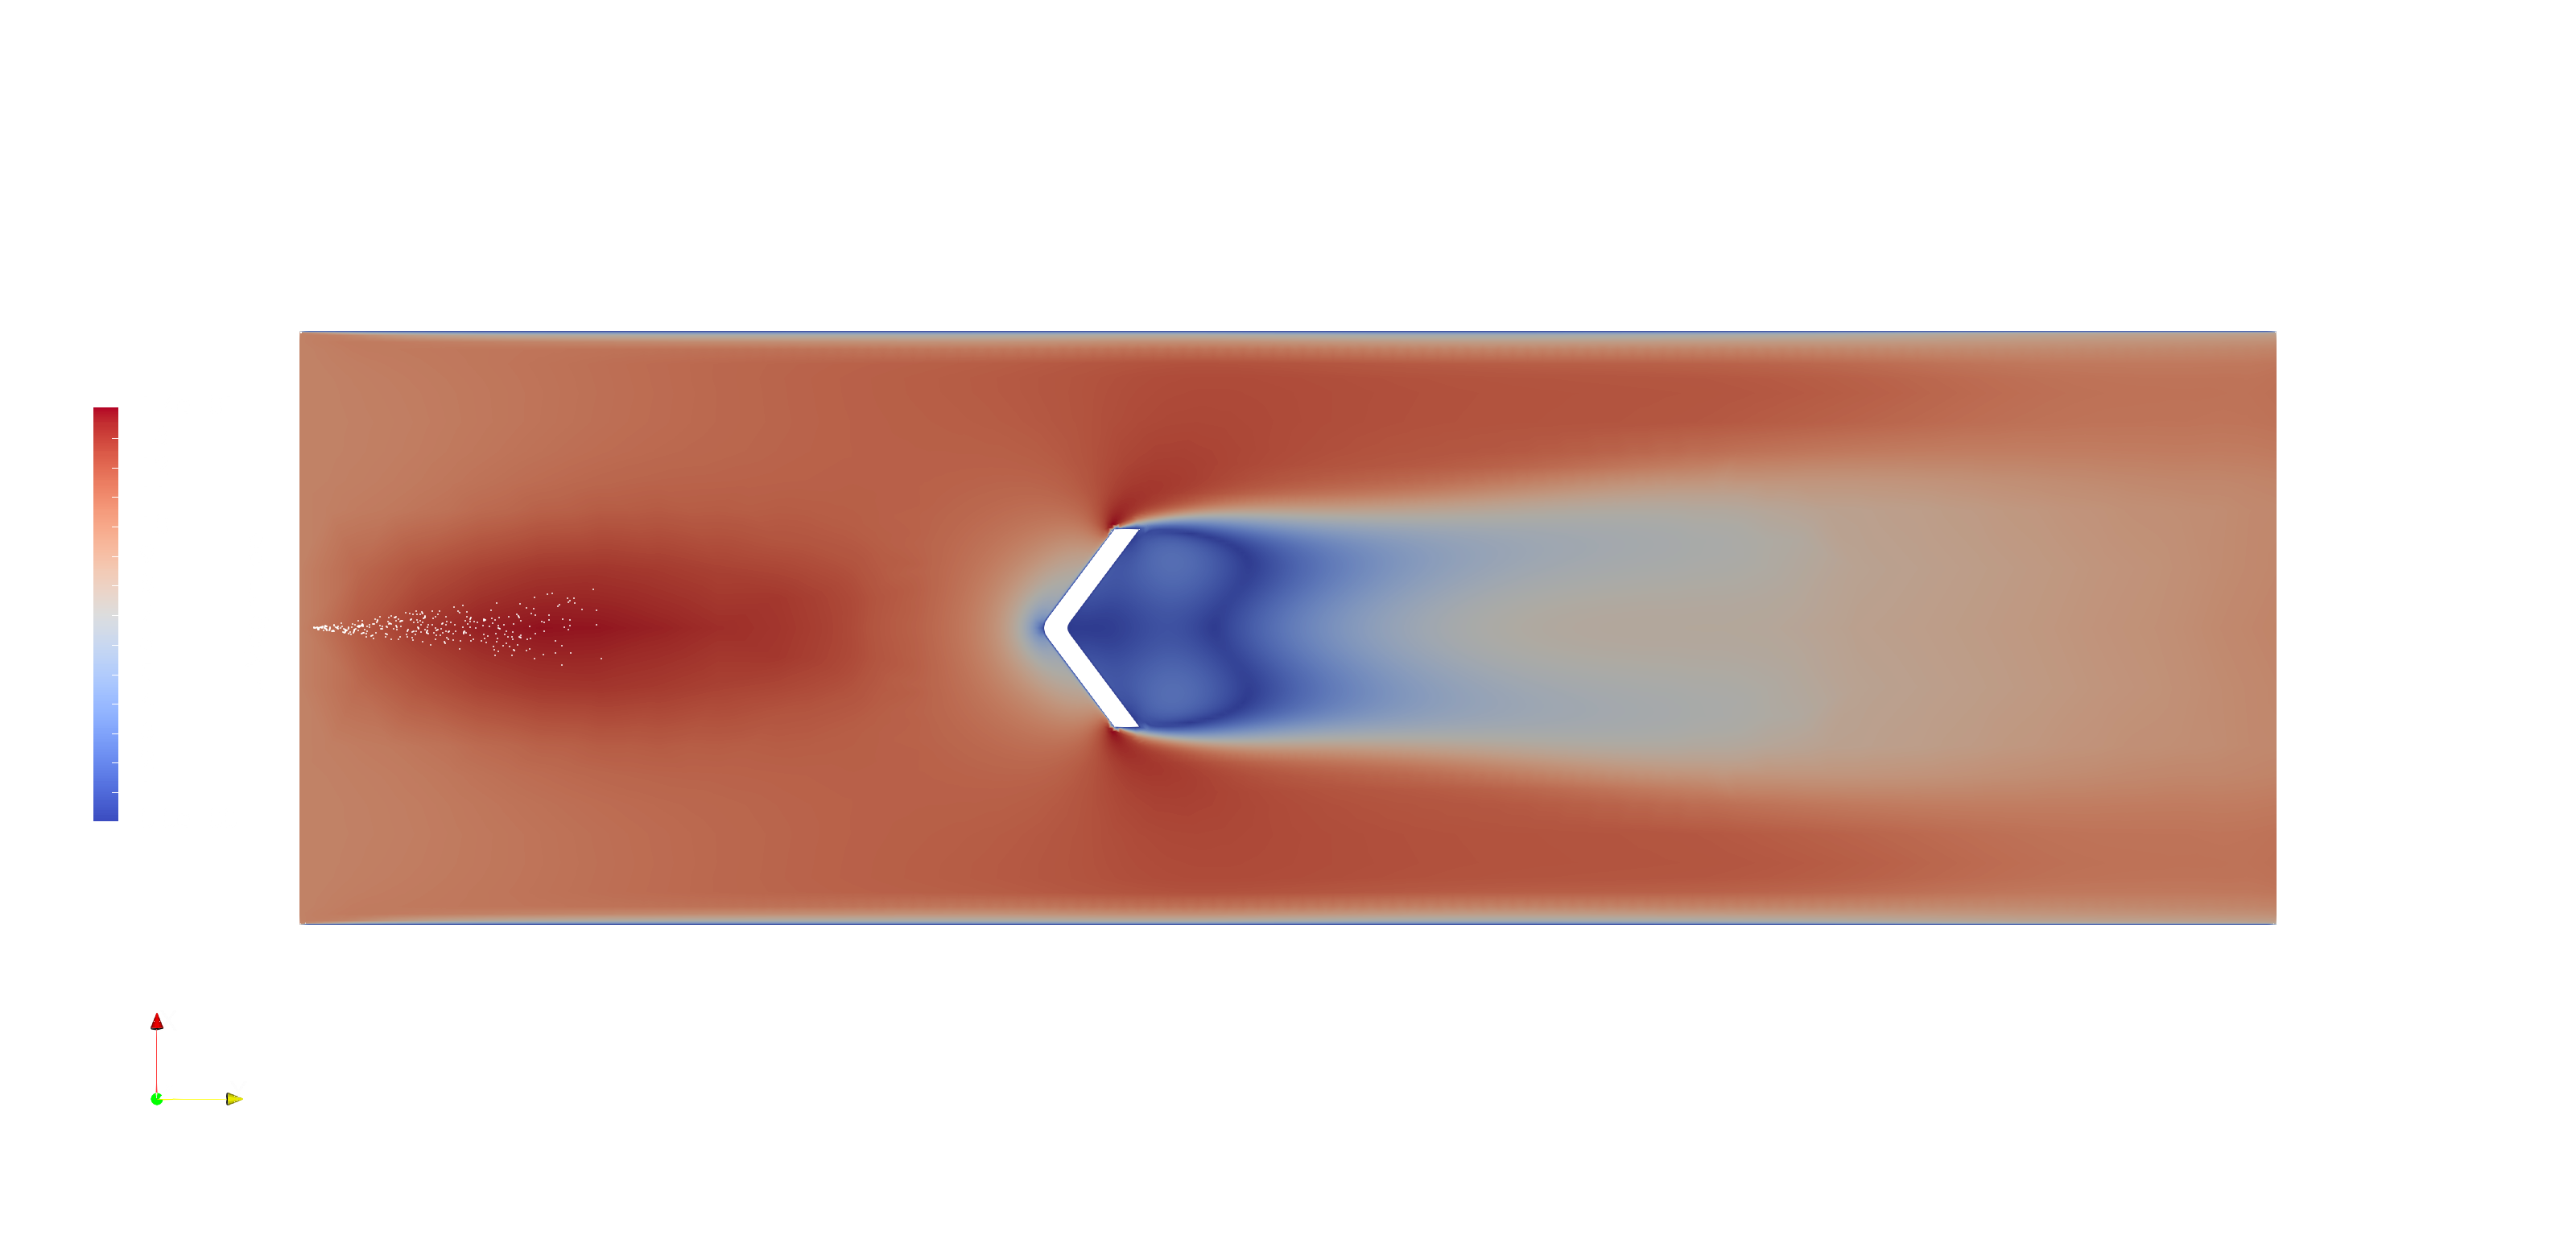
\includegraphics[width=0.8\textwidth]{latexFIGS/labAssignment/figU_02.png}
        \caption{3D reaction case: $|U|$ profile, $t = 0.02s$.}
    \end{figure}

    \begin{figure}[!ht]
        \centering
        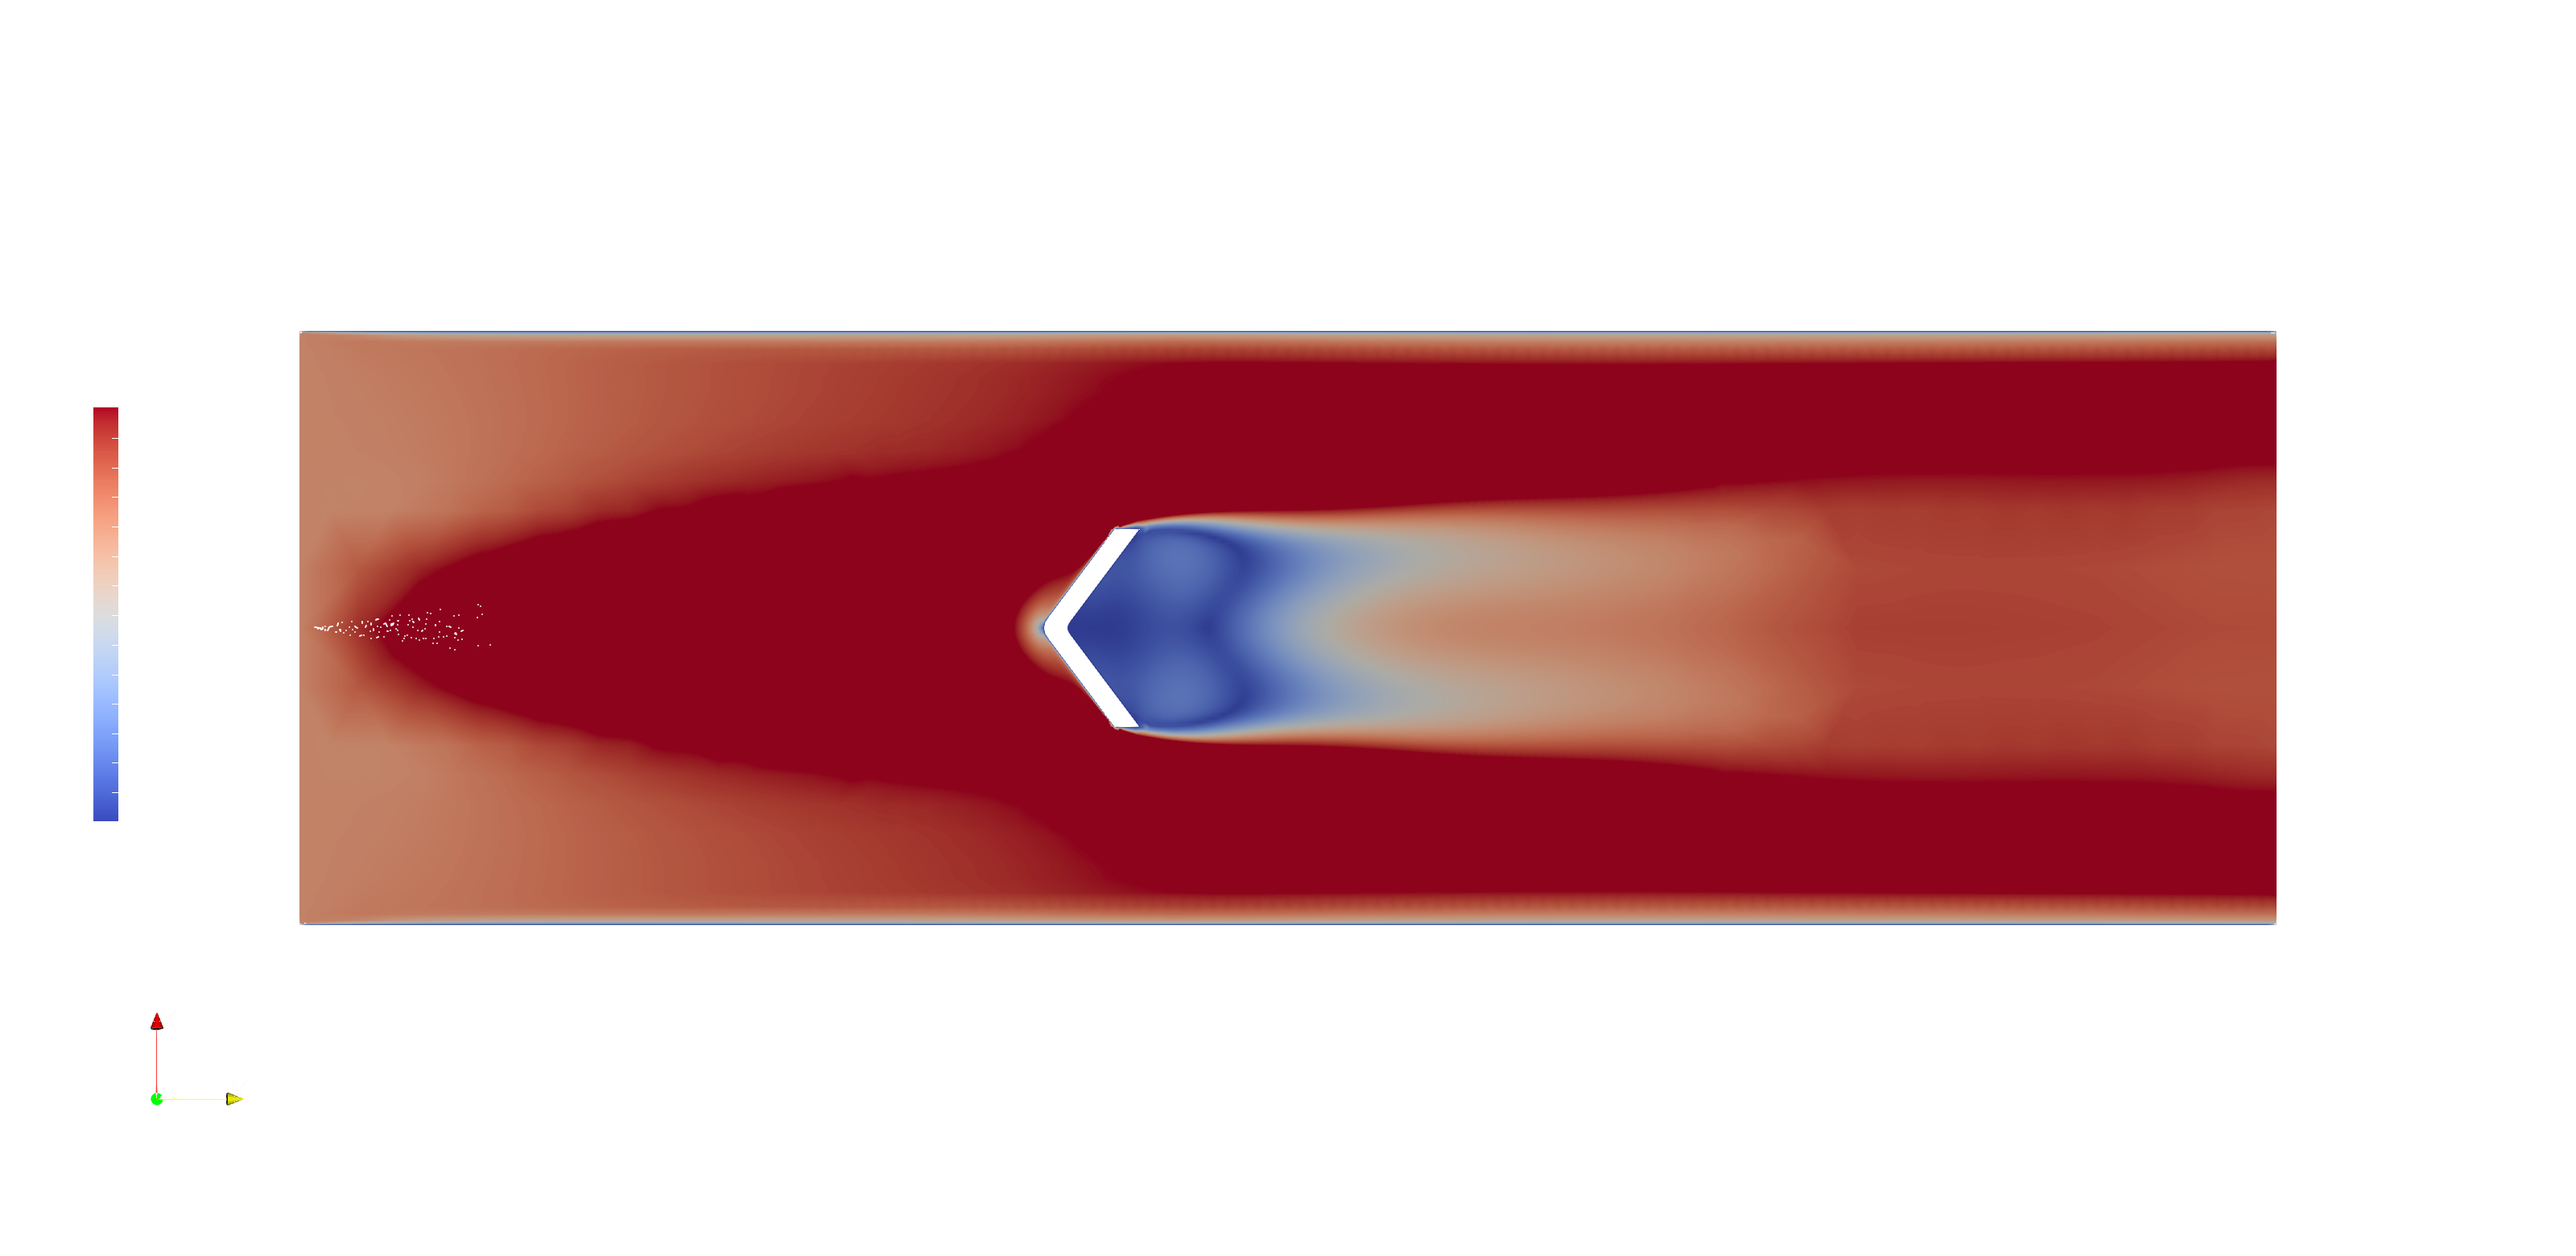
\includegraphics[width=0.8\textwidth]{latexFIGS/labAssignment/figU_05.png}
        \caption{3D reaction case: $|U|$ profile, $t = 0.05s$.}
    \end{figure}
    
    \begin{figure}[!ht]
        \centering
        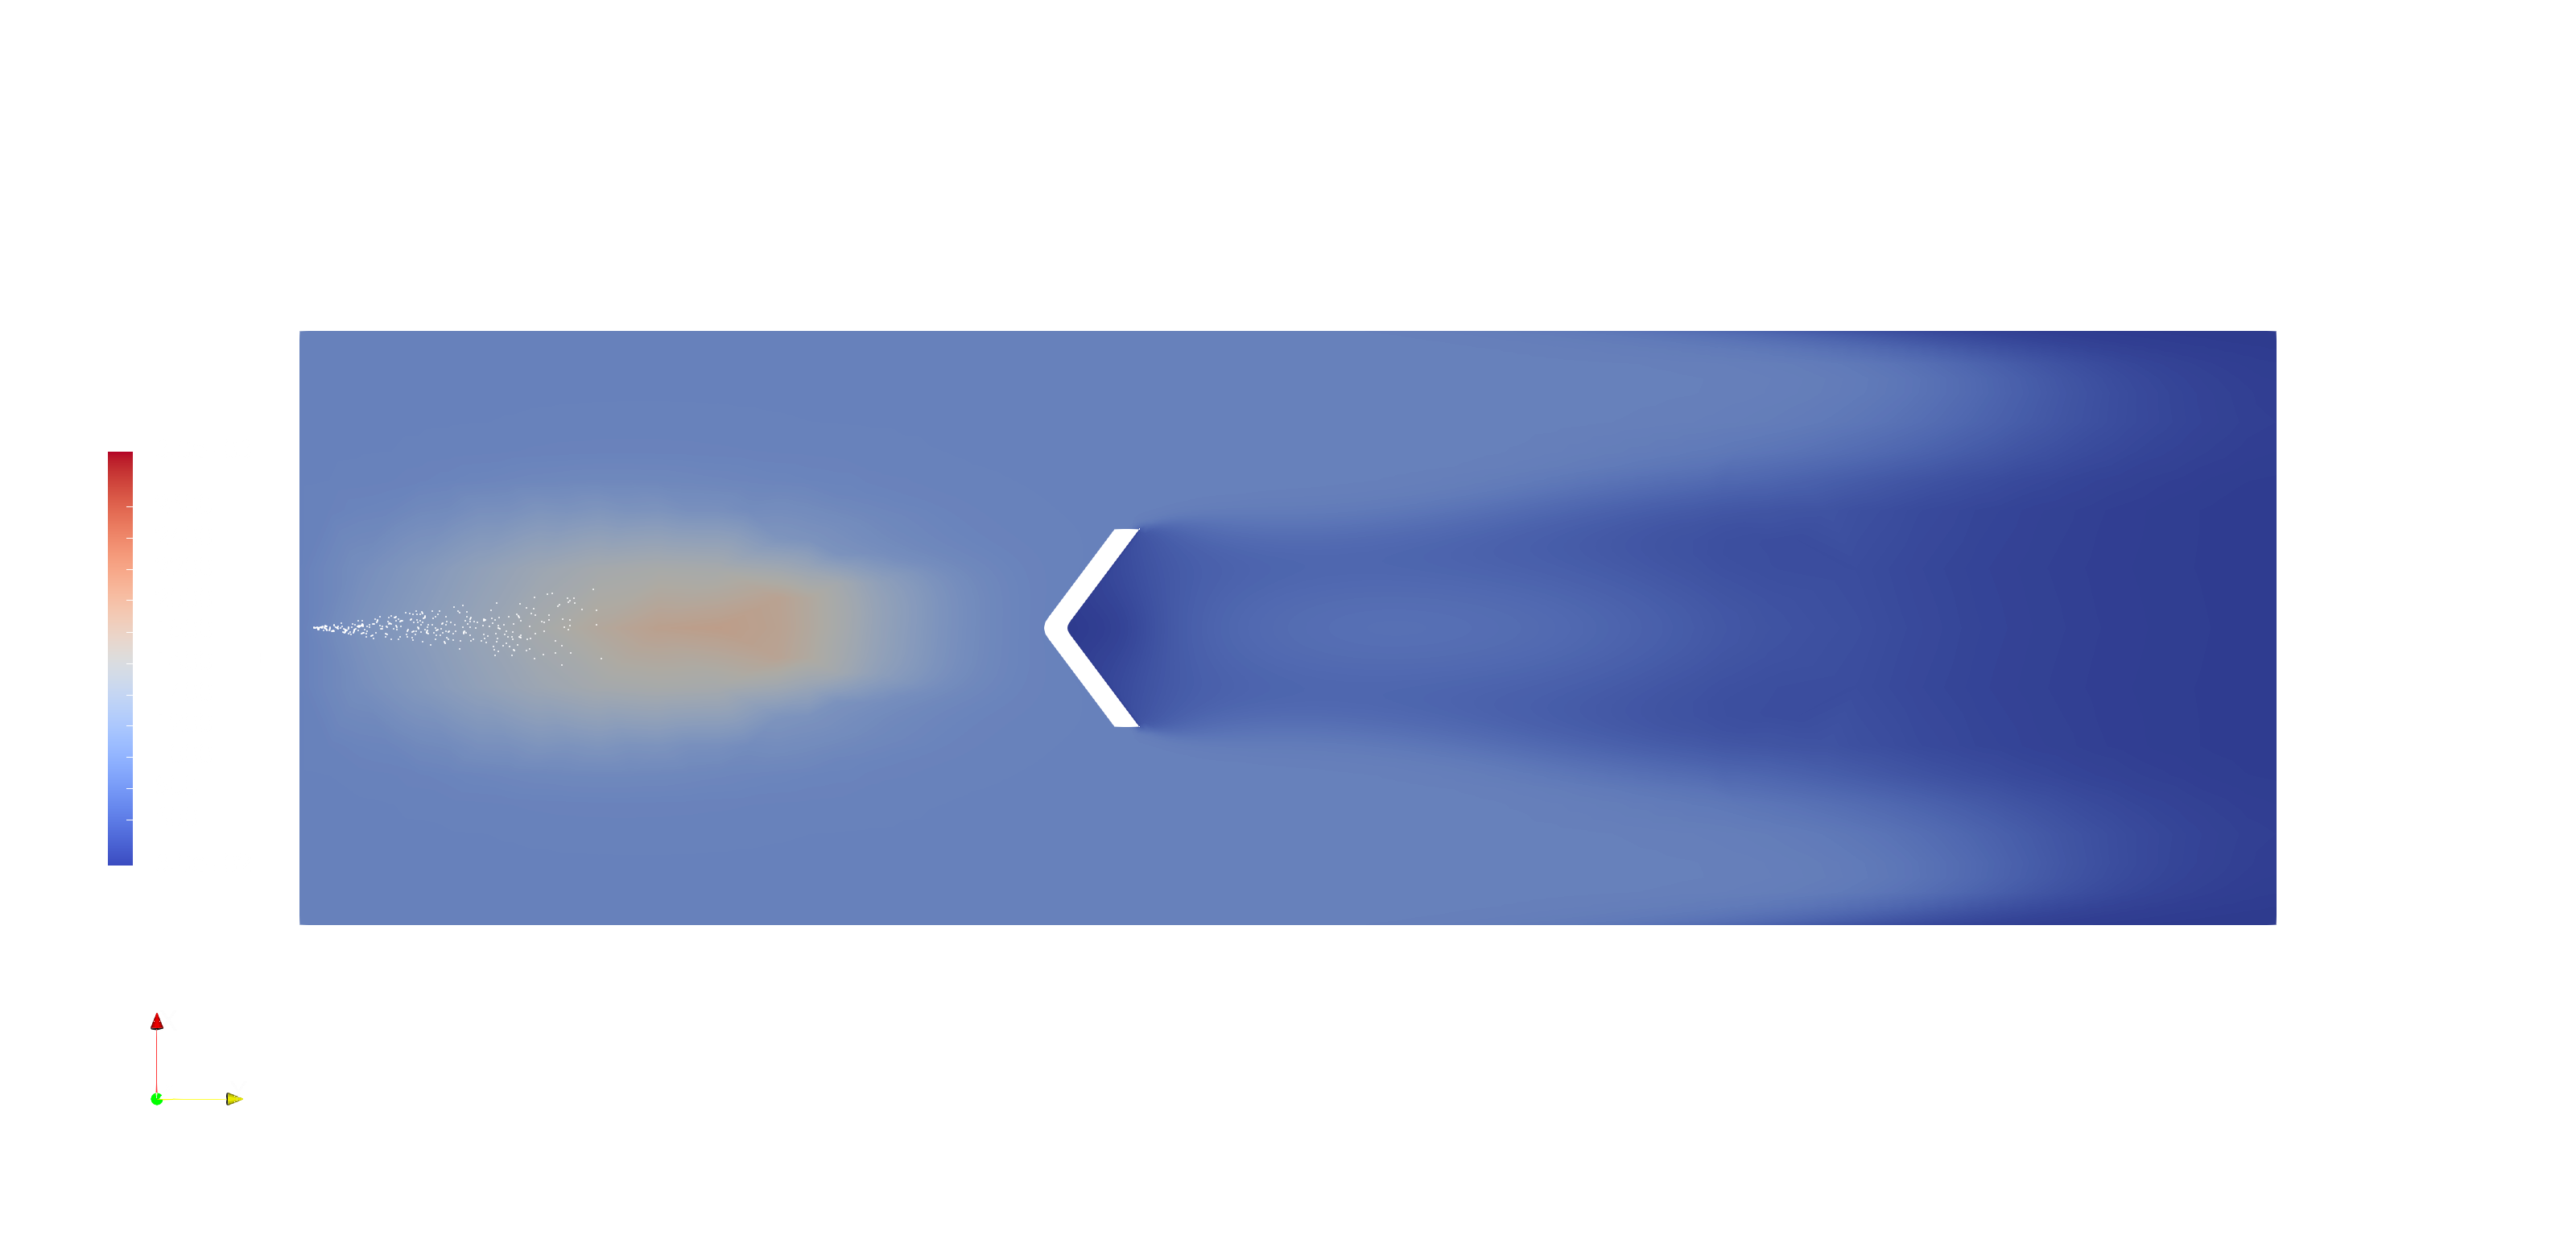
\includegraphics[width=0.8\textwidth]{latexFIGS/labAssignment/figT_02.png}
        \caption{3D reaction case: $T$ profile, $t = 0.02s$.}
    \end{figure}
    
    \begin{figure}[!ht]
        \centering
        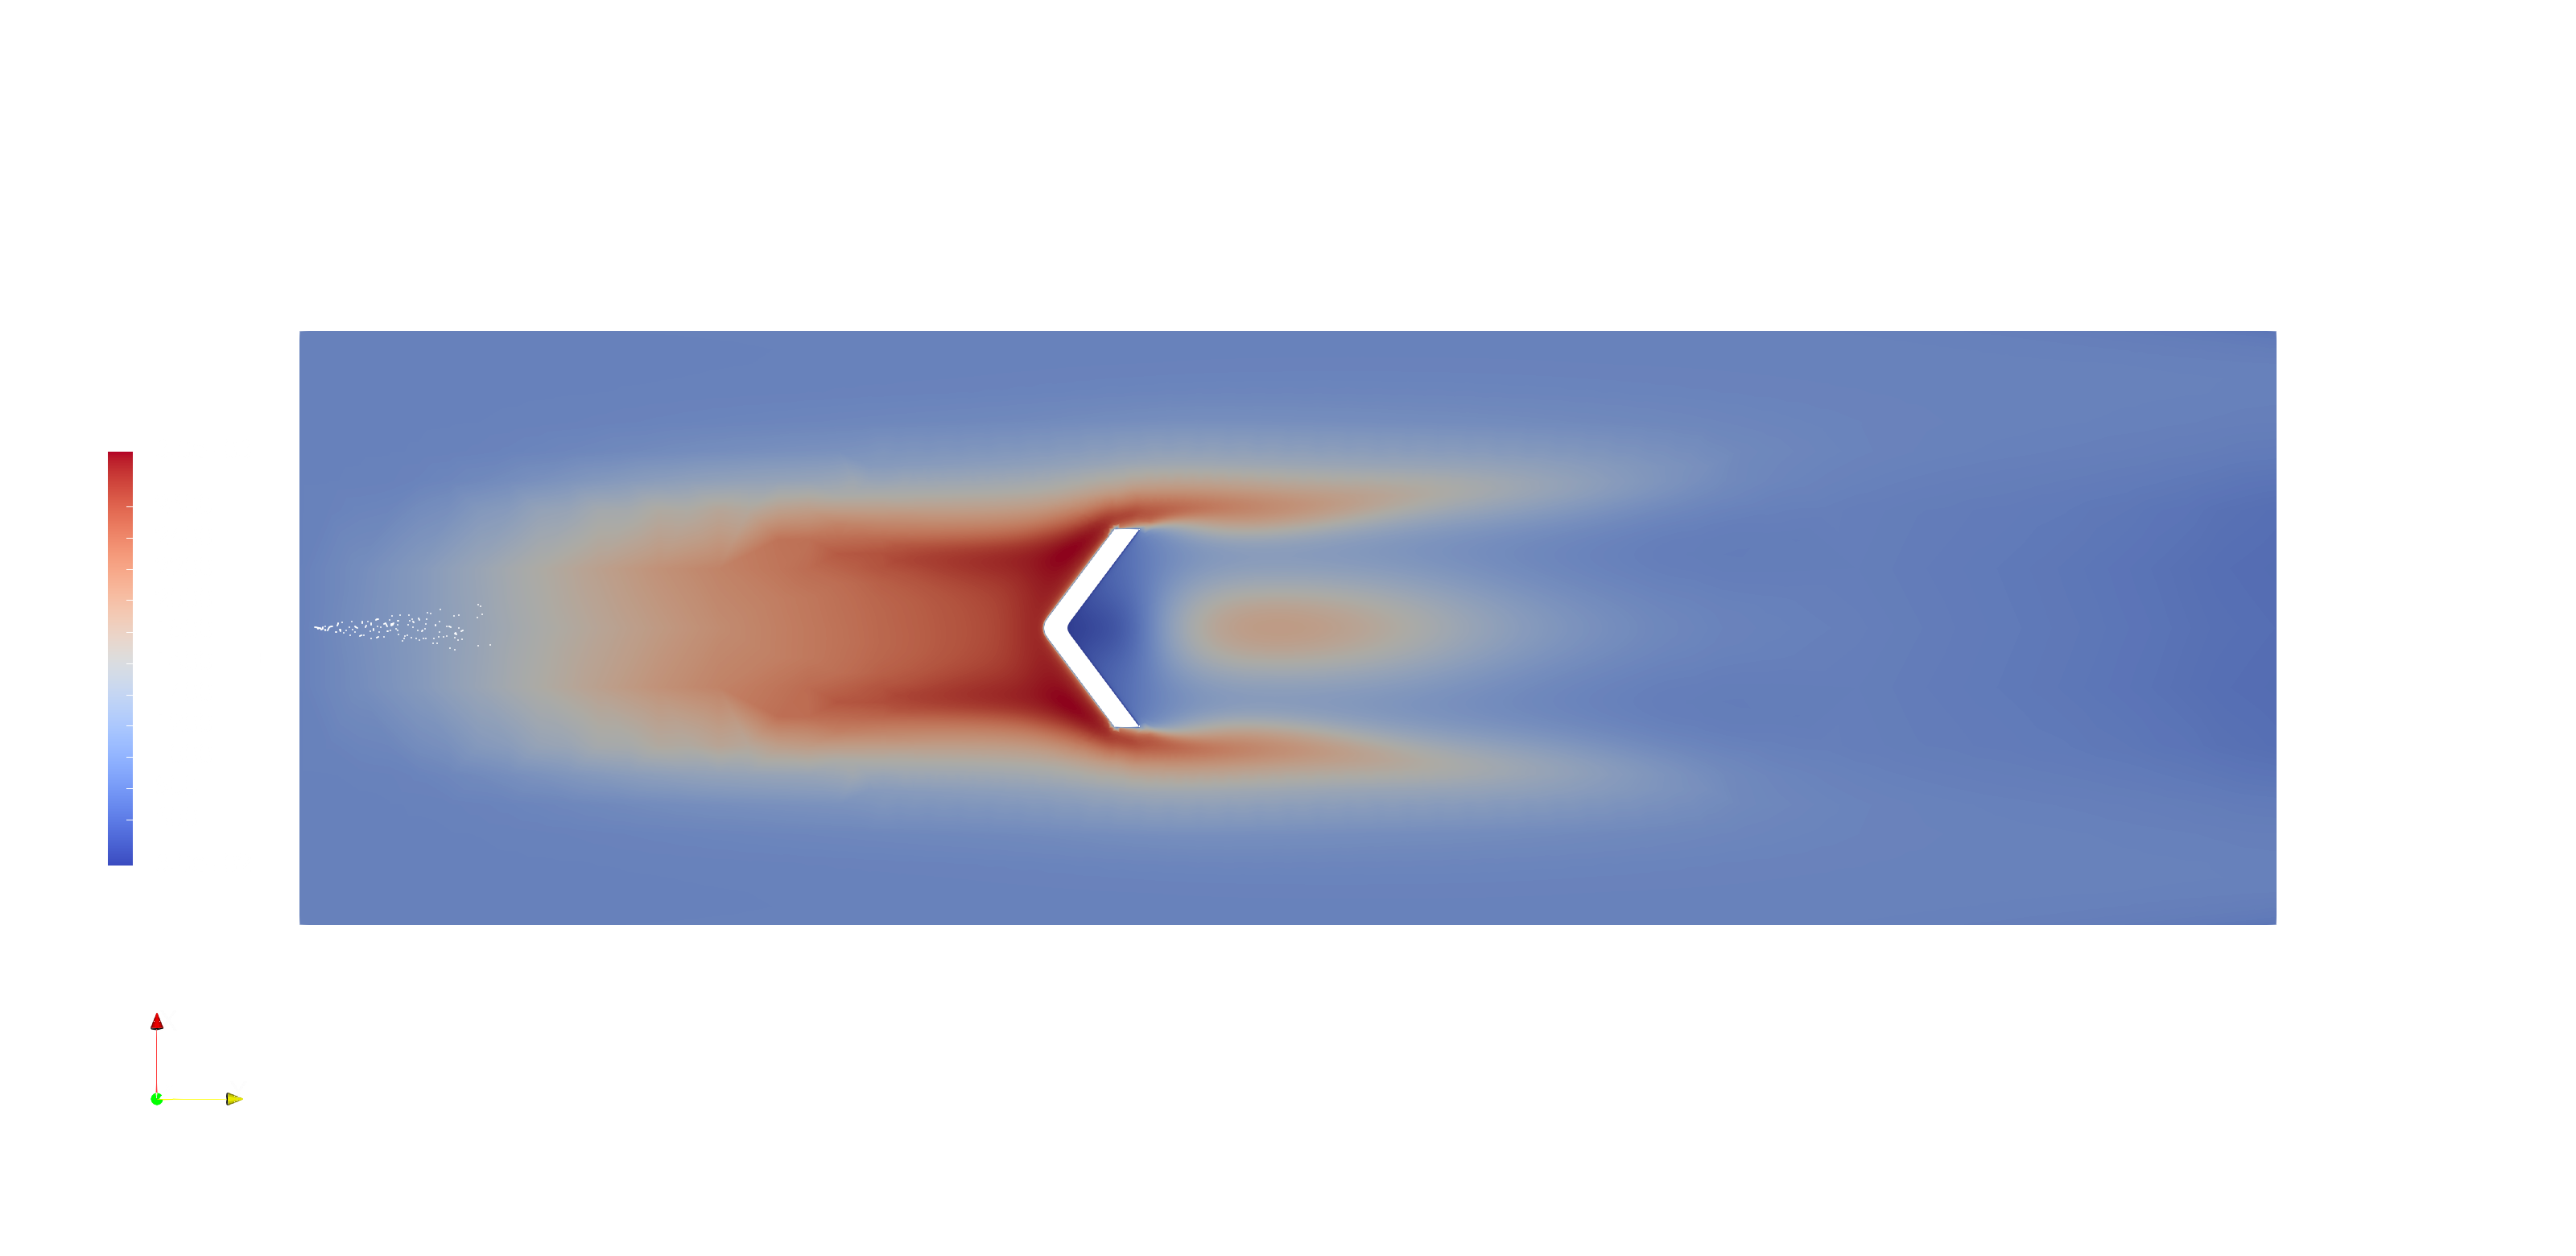
\includegraphics[width=0.8\textwidth]{latexFIGS/labAssignment/figT_05.png}
        \caption{3D reaction case: $T$ profile, $t = 0.05s$.}
    \end{figure}

    \begin{figure}[!ht]
        \centering
        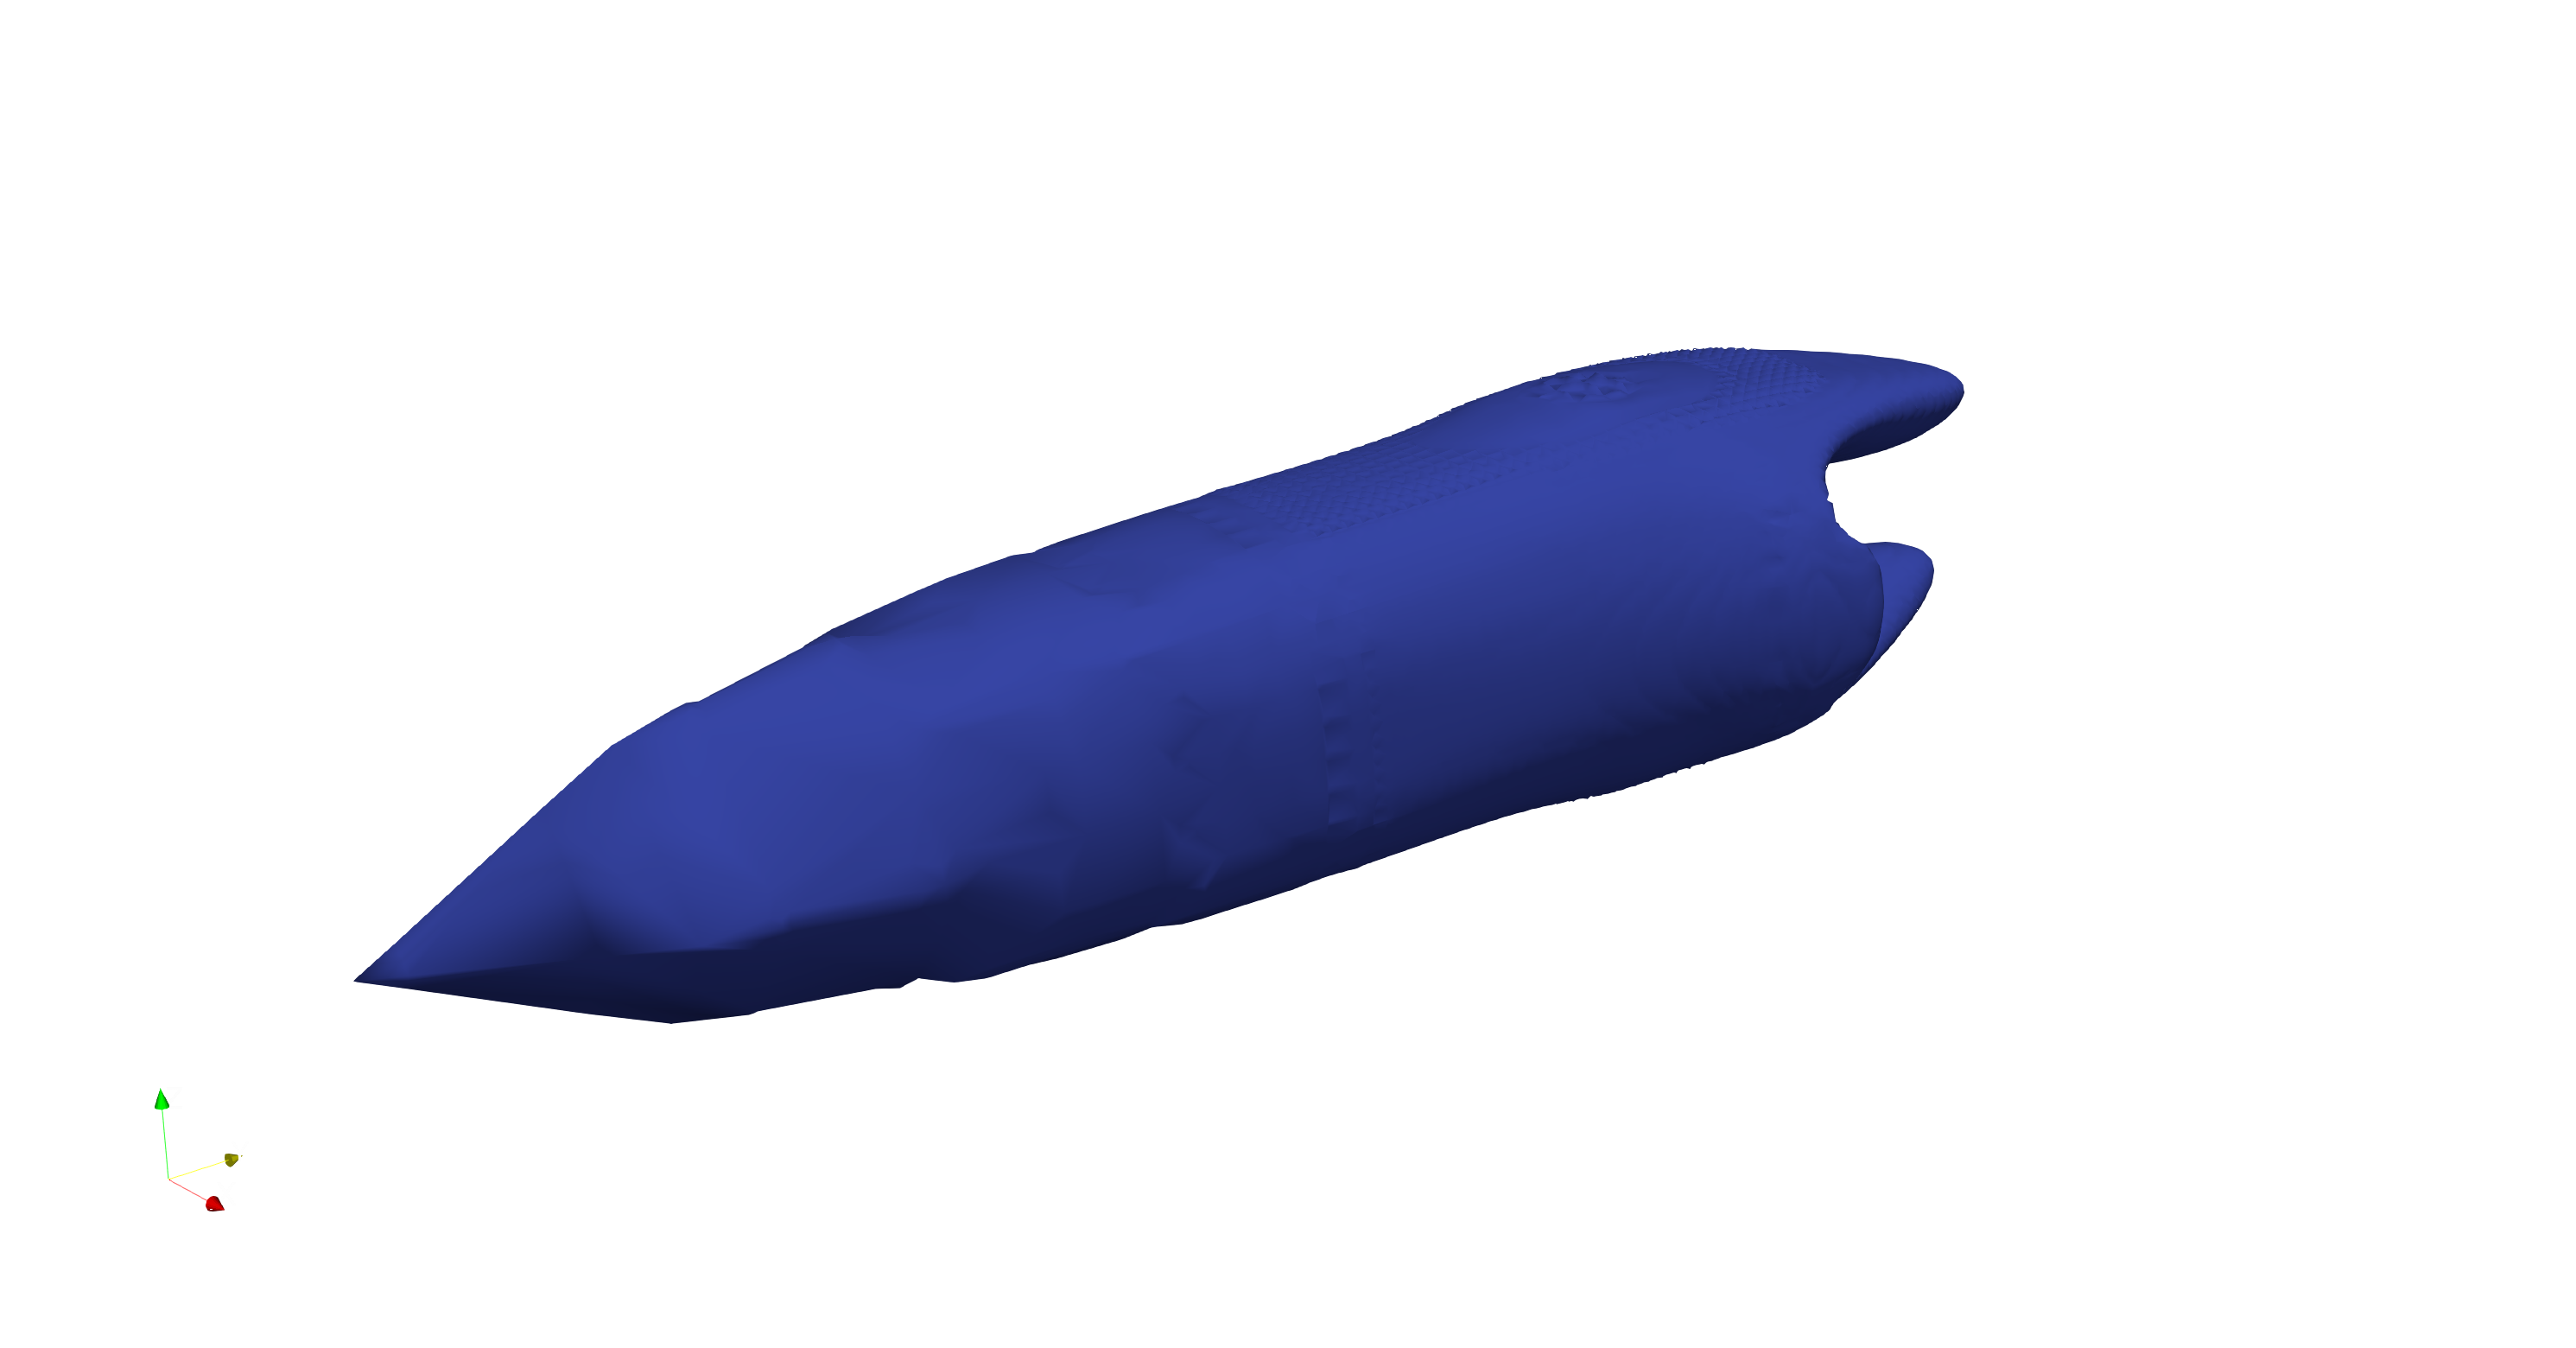
\includegraphics[width=0.8\textwidth]{latexFIGS/labAssignment/figAF.png}
        \cprotect\caption[3D reaction case: \verb|A/F| iso-surface, $t = 0.05s$]{3D reaction case: \verb|A/F| iso-surface, $t = 0.05s$. \newline ${C_7H_{16}}^{0.25} + 11 {O_2}^{1.5} \rightarrow 7 CO_2 + 8 H_2O$ \newline $\frac{A}{F} = \frac{O_2}{C_7H_{16}} \rightarrow surf\big( \frac{11 \cdot O_2^{1.5}}{{C_7H_{16}}^{0.25}} \big) = 1$}
    \end{figure}
    
    \clearpage
